\section{Results}
\label{sec:results}

\subsection{Comparison with baselines}
\label{sec:transfer}

\begin{table}[t]
\centering
\footnotesize
\setlength{\tabcolsep}{2.9pt}
\caption{Correspondence on both cohorts (number of lesions). Hit@$\tau$: selected point within $\tau$\,mm of the annotated earlier position; Reach@3: any candidate within 3\,mm; failures count as misses. Cand.: mean number of candidates scored per query (--: not applicable); $^\ast$mean after the gates. Bold: best method excluding the exhaustive reference.}
\label{tab:main}
\begin{tabular}{@{}lrrrrr@{}}
\toprule
Method & Cand. & Hit@2 & Hit@3 & Hit@4 & Reach@3 \\
\midrule
\multicolumn{6}{@{}l}{\emph{Independent staging cohort} ($n{=}440$)} \\
B-spline, lesion-incl.~\cite{rueckert1999} & -- & 199 & 243 & 267 & 243 \\
SAM standalone~\cite{yan2022sam} & -- & 36 & 99 & 184 & 396 \\
Siamese scorer, Relaxed 28 & 22$^\ast$ & 134 & 203 & 253 & 264 \\
Fit-only 28 & 28 & 157 & 205 & 237 & 221 \\
Diverse 28 & 28 & 197 & 245 & 275 & 274 \\
\textbf{\ours (ours)} & 363 & \textbf{259} & \textbf{289} & \textbf{306} & 348 \\
\cmidrule(l){1-6}
Exhaustive (reference) & 4,818 & 277 & 297 & 311 & 351 \\
\midrule
\multicolumn{6}{@{}l}{\emph{Screening cohort} ($n{=}309$)} \\
B-spline, lesion-incl.~\cite{rueckert1999} & -- & 170 & 211 & 231 & 211 \\
SAM standalone~\cite{yan2022sam} & -- & 27 & 80 & 147 & 308 \\
Siamese scorer, Relaxed 28 & 25$^\ast$ & 155 & 210 & 232 & 235 \\
Fit-only 28 & 28 & 141 & 175 & 196 & 189 \\
Diverse 28 & 28 & 164 & 212 & 230 & 242 \\
\textbf{\ours (ours)} & 360 & \textbf{207} & \textbf{244} & \textbf{255} & 289 \\
\cmidrule(l){1-6}
Exhaustive (reference) & 4,851 & 205 & 242 & 253 & 290 \\
\bottomrule
\end{tabular}
\end{table}


\begin{figure*}[!t]
\centering
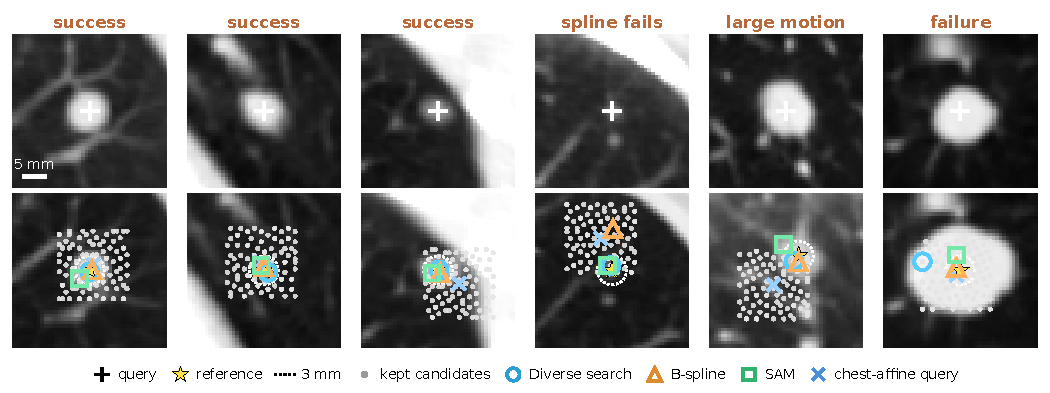
\includegraphics[width=\linewidth]{figures/qualitative.pdf}
\caption{Staging examples: three successes, a Spline failure, a large-motion case and a failure of \ours. Top: current CT with the query ($+$). Bottom: earlier CT with the reference (star, 3\,mm circle), retained candidates (dots) and each method's prediction.}
\label{fig:qualitative}

\end{figure*}

\Cref{tab:main} compares all methods on both cohorts; its rows are the Spline, SAM used standalone, our candidate lists scored by a learned Siamese network, the 28 best-fitting translations (Fit-only 28), diverse search stopped at 28 candidates (Diverse 28) or run to completion (\ours), and exhaustive scoring.
On the staging cohort, \ours places 289 of 440 predictions within 3\,mm (65.7\%), compared with 243 (55.2\%) for the Spline, a paired improvement of $+10.5$ points [3.6, 17.6]; on the screening cohort it reaches 244 of 309 (79.0\%) versus 211 (68.3\%), an improvement of $+10.7$ points [5.8, 15.4].
Both comparisons meet the criteria fixed before evaluation.
\Cref{fig:qualitative} shows typical cases, and the advantage holds at every tolerance, with every staging patient weighted equally ($+9.6$ [3.7, 15.9]) and in native earlier-scan coordinates ($+11.4$ [4.1, 18.9]) (supplement, \cref{fig:forest}).
SAM is far weaker as a standalone matcher (99 and 80 hits) even though its similarity map contains a correct location for most lesions, and the Siamese scorer reaches 203 and 210 hits on the Relaxed 28 lists, compared with 237 and 204 for our scorer on the same lists, so this learned scorer does not transfer to the staging cohort.

The gain over the Spline combines three differences, of which only the last is isolated (\cref{sec:diversity}): a wider search ($\pm7$ versus $\pm4.2$\,mm), the selection of the most lesion-like candidate rather than mapping the query (with the exact annotated query, the Spline improves from 211 to 239 screening hits while \ours remains at 243), and diverse search, which makes this wide, lesion-aware search affordable.
\Cref{tab:missmodes} shows where the remaining misses come from. Every miss of the Spline is unreachable by construction; \ours reduces unreachable staging lesions from 176 for the Relaxed 28 list to 92, leaving 59 selection misses, and on screening leaves 20 unreachable and 45 selection misses. Coverage therefore remains the larger limitation on staging, whereas selection dominates on screening.

\begin{table}[!t]
\centering
\footnotesize
\setlength{\tabcolsep}{2.6pt}
\caption{Where misses come from at 3\,mm. \emph{Unreach.}: no candidate within tolerance. \emph{Missel.}: a candidate was within tolerance but the scorer chose another. The Spline returns a single point, so all its misses are unreachable. Diverse search removes most unreachable misses; SAM's field reaches almost everything but rarely selects correctly. Bold: most hits excluding the exhaustive reference.}
\label{tab:missmodes}
\begin{tabular}{@{}lcccccc@{}}
\toprule
& \multicolumn{3}{c}{Staging ($n{=}440$)} & \multicolumn{3}{c}{Screening ($n{=}309$)} \\
\cmidrule(lr){2-4}\cmidrule(l){5-7}
Method & Hits & Unreach. & Missel. & Hits & Unreach. & Missel. \\
\midrule
B-spline & 243 & 197 & 0 & 211 & 98 & 0 \\
SAM standalone & 99 & 44 & 297 & 80 & 1 & 228 \\
Relaxed 28 & 237 & 176 & 27 & 204 & 74 & 31 \\
\quad + Siamese scorer & 203 & 176 & 61 & 210 & 74 & 25 \\
\textbf{\ours} & \textbf{289} & 92 & 59 & \textbf{244} & 20 & 45 \\
\cmidrule(l){1-7}
Exhaustive (reference) & 297 & 89 & 54 & 242 & 19 & 48 \\
\bottomrule
\end{tabular}
\end{table}



\subsection{Effect of diverse search at a fixed budget}
\label{sec:diversity}
\Cref{tab:contrasts} isolates candidate allocation by changing only the list, with the same order, grid and scorer.
At a budget of 28, enforcing a minimum distance of 2.1\,mm raises reach from 221 to 274 staging lesions and from 189 to 242 screening lesions, and raises hits from 205 to 245 ($+9.1$ points [6.0, 12.2]) and from 175 to 212 ($+12.0$ points [7.5, 16.4]), at an extra cost of 22\,ms per query.
The gain persists with relaxed gates, where diverse search at 28 adds 7.5 [4.7, 10.7] and 9.4 [5.3, 13.4] points. \Cref{fig:attribution} decomposes these gains with \cref{eq:decomp}. Diverse search makes 54 staging and 56 screening lesions newly reachable, of which the scorer selects 45 and 41, while choices on lesions reachable by both lists change by a net $-4$ in each cohort.
The improvement is therefore entirely due to coverage.
Equal-budget controls (supplement, \cref{sec:alloc}) show that spatial spread alone does not suffice: random and farthest-point lists of 28 candidates give $-24.09$ and $-14.55$ points relative to Diverse 28 on staging and $-29.47$ and $-16.83$ on screening, whereas a fit-informed spatial stratification performs on par ($+0.23$ [$-2.46$, 3.23] and $-1.29$ [$-5.02$, 2.48]).
The gain therefore stems from combining anatomical fit with spatial coverage, of which diverse search is one simple instance.
Relative to $r = 2.1$\,mm, a radius of 1.4\,mm changes hits by $-3.86$ points [$-6.46$, $-1.29$] and $-5.50$ [$-8.62$, $-2.40$], and a radius of 2.8\,mm by $+2.05$ [$-0.75$, 5.03] and $-1.94$ [$-4.98$, 1.05], so neither alternative improves both cohorts.


\begin{table}[!t]
\centering
\footnotesize
\setlength{\tabcolsep}{2.2pt}
\begin{tabular}{@{}llccc@{}}
\toprule
& Change & Reach & Hits & $+$/$-$ \\
\midrule
\multirow{7}{*}{\rotatebox{90}{Staging}}
& Diversify at 28 & 221$\to$274 & 205$\to$245 & 51/11 \\
& Gated, $K$ 7$\to$28 (direct) & 202$\to$241 & 192$\to$219 & 34/7 \\
& Gated, $K$ 7$\to$28 (SAM) & 202$\to$241 & 144$\to$139 & 17/22 \\
& Gated 28, wider lattice & 239$\to$241 & 220$\to$219 & 15/16 \\
& Relaxed, 28$\to$all & 264$\to$300 & 237$\to$264 & 33/6 \\
& Remove gates, all & 300$\to$348 & 264$\to$289 & 30/5 \\
& \ours$\to$exhaustive & 348$\to$351 & 289$\to$297 & 12/4 \\
\midrule
\multirow{7}{*}{\rotatebox{90}{Screening}}
& Diversify at 28 & 189$\to$242 & 175$\to$212 & 44/7 \\
& Gated, $K$ 7$\to$28 (direct) & 185$\to$220 & 167$\to$195 & 28/0 \\
& Gated, $K$ 7$\to$28 (SAM) & 185$\to$220 & 121$\to$118 & 23/26 \\
& Gated 28, wider lattice & 220$\to$220 & 193$\to$195 & 9/7 \\
& Relaxed, 28$\to$all & 235$\to$257 & 204$\to$217 & 14/1 \\
& Remove gates, all & 257$\to$289 & 217$\to$244 & 29/2 \\
& \ours$\to$exhaustive & 289$\to$290 & 244$\to$242 & 6/8 \\
\bottomrule
\end{tabular}
\caption{Paired changes to the candidate list at 3\,mm on all 440 staging and 309 screening lesions. $+$/$-$ counts lesions that become hits / stop being hits. Differences in points with 95\% intervals are plotted in supplement Fig.~S3.}
\label{tab:contrasts}
\end{table}


\begin{figure}[!t]
\centering
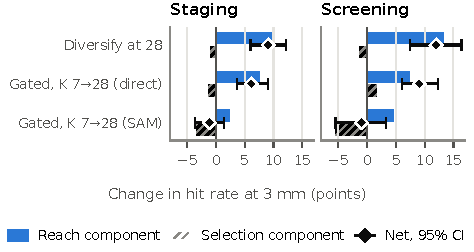
\includegraphics[width=\linewidth]{figures/reach_selection.pdf}
\caption{Where additional hits come from (\cref{eq:decomp}): reach term (blue), selection term (hatched) and net change with 95\% interval (black). Gains come through reach; SAM loses on shared lesions.}
\label{fig:attribution}
\end{figure}

Supplement \cref{fig:budget} shows reach and hits as the budget grows.
Each doubling of a diverse budget increases reach, and hits closely follow reach.
In contrast, Gated $K$ gains little beyond $K{=}28$, because its gates have already removed the neighborhoods that contain the lesion.
With relaxed gates, replacing the budget of 28 by the complete list raises hits from 237 to 264 (staging) and from 204 to 217 (screening), and removing the remaining gates adds another 48 and 32 reachable lesions and 25 and 27 hits.
Anatomical fit is therefore more useful as a soft term in the score (\cref{eq:direct}) than as a hard filter on the list.
Run to completion, \ours reaches 348 of the 351 lesions reachable on the full lattice in staging and 289 of 290 in screening, while scoring about 360 of the 4,851 translations.
Exhaustive scoring remains the most accurate option on staging (297 versus 289 hits; $+1.8$ points [0.2, 3.5]), whereas \ours is two hits ahead on screening (244 versus 242); consistent with the coverage bound (\cref{eq:coverage}), the staging gap grows to 18 hits at 2\,mm and shrinks to five at 4\,mm.
Scoring only 7.5\% of the translations matters most when scoring dominates the cost, as it would with a neural scorer: in the fixed-budget replay, scoring takes 0.201 of the 0.265\,s of exhaustive search.
\label{sec:query}
Our queries are perturbed annotations (\cref{sec:evaluation}), so we examine how the gain depends on query error.
\begin{figure}[!t]
\centering
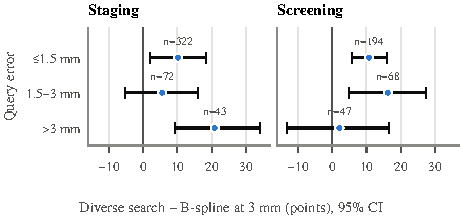
\includegraphics[width=\linewidth]{figures/query_bands.pdf}
\caption{Gain over the Spline by query error, with 95\% patient-level intervals; $n$: lesions per band. The gain is present even for accurate queries.}
\label{fig:bands}
\end{figure}
\Cref{fig:bands} groups lesions by the distance between the query $p$ and the annotated current position.
The gain is already present for well-localized queries: within 1.5\,mm, \ours hits 238 of 322 staging lesions versus 205 for the Spline ($+10.2$ points [2.1, 18.4]) and 178 versus 157 of 194 screening lesions ($+10.8$ [5.8, 16.0]); this band accounts for 33 of the 46 net staging gains and 21 of the 33 screening gains.
When the screening cohort is rerun with the exact annotated position as the query, the Spline improves from 211 to 239 hits while \ours remains at 243.
On screening, a large part of the advantage is therefore robustness to an imprecise query, which matters whenever the query comes from a click or a detector (supplement, \cref{tab:query-bands}). Additional reach is useful only if the scorer can exploit it.
Increasing the budget of Gated $K$ from 7 to 28 raises hits from 192 to 219 on staging ($+6.1$ points [3.6, 9.1]) and from 167 to 195 on screening ($+9.1$ points [6.0, 12.3]), both above the margin fixed before evaluation.
Widening the lattice at a fixed budget of 28 does not help (intervals include zero), so the number and placement of the retained candidates, rather than the extent of the lattice, drive the gain.
On identical expanded lists, our scorer selects 33 of the 39 newly reachable staging lesions, whereas SAM selects only 10 and loses 15 hits on the 202 lesions reachable by both lists (\cref{fig:attribution}).
The budget effect favors our scorer over SAM by 7.3 points [4.4, 10.4] on staging and 10.0 [5.4, 14.8] on screening.
Coverage and selection are therefore complementary: a wider candidate list helps only when the scorer can distinguish the lesion from anatomically similar structures.
\begin{table}[!t]
\centering
\footnotesize
\setlength{\tabcolsep}{3pt}
\caption{Median local time per query (s) on prepared crops, one CPU thread, matched workloads of 24 staging and 32 screening queries. The matched comparison is a single timing pass per method; the fixed-budget replay takes the median of three randomized repetitions. SAM runs on a GPU (0.033\,s per screening query) and is not comparable. Supplement, \cref{tab:timing-v6,tab:fixed-budget-timing}.}
\label{tab:timing}
\begin{tabular}{@{}lcccc@{}}
\toprule
& \multicolumn{2}{c}{Matched comparison} & \multicolumn{2}{c}{Fixed-budget replay} \\
\cmidrule(lr){2-3}\cmidrule(l){4-5}
Method & Staging & Screening & Staging & Screening \\
\midrule
B-spline & 3.617 & 3.866 & -- & -- \\
Siamese, Relaxed 28 & 0.106 & 0.082 & -- & -- \\
Fit-only 28 & -- & -- & 0.098 & 0.101 \\
Diverse 28 & -- & -- & 0.120 & 0.120 \\
Diverse 112 & -- & -- & 0.142 & 0.144 \\
\textbf{\ours} & 0.194 & 0.185 & 0.190 & 0.190 \\
Exhaustive & 0.956 & 0.256 & 0.265 & 0.265 \\
\bottomrule
\end{tabular}
\end{table}
In the matched comparison (prepared crops, one CPU thread, 24 staging and 32 screening queries; \cref{tab:timing}), the median local time of \ours is 0.194\,s versus 3.617\,s for the Spline on staging (18.6$\times$ faster) and 0.185 versus 3.866\,s on screening (20.9$\times$).
Supplement \cref{fig:speed} plots accuracy against local time in the fixed-budget replay, where a budget of 112 yields 278 staging hits at 0.142\,s.
In this single-pass matched comparison, exhaustive scoring took 0.956\,s on staging (4.9$\times$ the time of \ours) but 0.256\,s on screening (1.4$\times$), whereas the fixed-budget replay gives 0.265\,s on both cohorts, so its measured relative cost depends on the timing protocol.
End to end, the shared chest alignment dominates: with one query per screening pair, \ours takes 29.36\,s versus 32.87\,s for the Spline, and with two queries sharing one alignment, 14.88 versus 19.38\,s per query; the relative saving grows as more lesions share an alignment.
